\documentclass[12pt]{article}
\usepackage{arxiv}
\usepackage[utf8]{inputenc}
\usepackage[T1]{fontenc}
\usepackage{lmodern}
\usepackage{geometry}
\usepackage{hyperref}
\usepackage{graphicx}
\usepackage{booktabs}
\usepackage{array}
\usepackage{longtable}
\usepackage{enumitem}
\geometry{margin=1in}

  \title{Laporan Proyek Mata Kuliah Teknologi Blockchain \\ \Large\textbf{Pengembangan Aegis: Crowdfunding Berbasis Milestone di Ethereum}}

\author{%
Rifqi Ramadhan (2206062964)\\
George Wiliam Thomas Gonata (2206024253)\\
Samuel Tanaka Sibarani (2206059710)\\
Prof. Dr. Ir. Riri Fitri Sari, M.M., M.Sc.\\
\textit{Departemen Teknik Elektro, Fakultas Teknik, Universitas Indonesia}\\
Juni 2026
}

\date{}

\begin{document}
\begin{center}

\includegraphics[width=0.25\textwidth]{logo_ui.png}
\end{center}
\vspace{0.5em}
\maketitle

\begin{abstract}
Laporan ini menjelaskan perkembangan terkini proyek \textit{Aegis}, sebuah platform crowdfunding berbasis blockchain dengan mekanisme pelepasan dana per-milestone. Fokus implementasi saat ini adalah memastikan alur inti berjalan end-to-end: penciptaan proyek, penggalangan dana berbasis ETH, pelaporan milestone, voting oleh backer berdasarkan kontribusi, dan pelepasan dana otomatis. Sistem dibangun melalui smart contract inti (Factory + Project) dan antarmuka pengguna berbasis React yang terhubung lewat MetaMask. Fitur lanjutan seperti escrow stablecoin, integrasi DeFi yield, serta governance token terpisah masih berada di luar scope implementasi saat ini. Laporan ini menyajikan desain sistem, status implementasi, pembagian tugas tim, dan timeline pengembangan secara lebih naratif.
\end{abstract}

\section*{Abstract (English)}
This report describes the current progress of \textit{Aegis}, a blockchain-based crowdfunding platform with milestone-based fund releases. The current implementation focuses on the end-to-end flow: project creation, ETH funding, milestone reporting, contribution-weighted voting, and automatic fund release. The system is composed of core smart contracts (Factory + Project) and a React frontend integrated through MetaMask. Advanced features such as stablecoin escrow, DeFi yield, and a separate governance token are out of scope for the current implementation. We present the system design, implementation status, team responsibilities, and a detailed development timeline in a narrative form.

\newpage
	\tableofcontents
\listoffigures
\listoftables

\section*{Daftar Singkatan dan Istilah}
\begin{itemize}[leftmargin=1.2em]
  \item ETH: Ether (native asset jaringan Ethereum)
  \item DApp: Decentralized Application
  \item EOA: Externally Owned Account
  \item UI/UX: User Interface/User Experience
  \item Web3: Ekosistem aplikasi terdesentralisasi berbasis blockchain
\end{itemize}

\newpage

\section{BAB 1. PENDAHULUAN}
\subsection{Latar Belakang}
Crowdfunding tradisional menghadapi tantangan transparansi, potensi fraud, serta pelepasan dana yang tidak terkontrol. Dalam praktiknya, backer sering kali hanya memiliki sedikit visibilitas terhadap progres proyek, sehingga keputusan pendanaan berikutnya berisiko tidak berbasis bukti. Aegis hadir sebagai prototipe yang memindahkan mekanisme akuntabilitas ke smart contract: dana dikunci di kontrak, kreator mengirim laporan milestone, dan komunitas memutuskan kelayakan pencairan.

\subsection{Identifikasi Masalah}
Permasalahan utama yang teridentifikasi adalah ketidakjelasan progres proyek, mekanisme verifikasi yang lemah, serta keterbatasan kontrol komunitas terhadap pencairan dana. Dalam konteks ini, solusi digital berbasis blockchain dipilih untuk memberikan jejak audit dan mekanisme verifikasi yang transparan.

\subsection{Rumusan Masalah}
Rumusan masalah yang dijawab melalui proyek ini adalah: (1) bagaimana merancang sistem crowdfunding berbasis milestone yang transparan, (2) bagaimana memastikan dana hanya dilepas setelah bukti kemajuan diverifikasi, dan (3) bagaimana menghadirkan mekanisme voting yang sederhana namun adil bagi backer.

\subsection{Tujuan Project}
Tujuan utama proyek adalah membangun prototipe sistem crowdfunding berbasis blockchain yang menjalankan alur end-to-end, menyediakan transparansi status, serta meminimalkan risiko pencairan dana tanpa bukti.

\subsection{Manfaat Project}
Manfaat yang diharapkan adalah peningkatan akuntabilitas kreator, transparansi bagi backer, serta dasar implementasi governance yang dapat dikembangkan ke tahap token-based voting di masa depan.

\subsection{Ruang Lingkup}
Ruang lingkup mencakup kontrak inti (Factory + Project), kontribusi ETH, pelaporan milestone, voting berbasis kontribusi, dan UI berbasis React. Fitur lanjutan seperti stablecoin escrow dan DeFi yield tidak diimplementasikan pada tahap ini.

\subsection{Metodologi Pengembangan}
Pengembangan dilakukan secara iteratif dengan fokus pada prototyping: merancang kontrak, membangun UI, menguji alur utama, dan memperbaiki pengalaman pengguna berdasarkan hasil pengujian lokal.

\subsection{Sistematika Penulisan}
Laporan ini disusun ke dalam sembilan bab: pendahuluan, tinjauan pustaka, analisis masalah dan kebutuhan, desain solusi, manajemen proyek, implementasi, pengujian dan evaluasi, hasil dan tampilan, serta kesimpulan dan saran.

\section{BAB 2. TINJAUAN PUSTAKA}
\subsection{Definisi Blockchain}
Blockchain adalah ledger terdistribusi yang menyimpan transaksi secara transparan dan immutable. Karakteristik ini relevan untuk sistem crowdfunding karena memungkinkan pelacakan dana dan status proyek secara terbuka.

\subsection{Smart Contract}
Smart contract adalah program on-chain yang mengeksekusi aturan tanpa perantara. Dalam Aegis, kontrak berperan sebagai escrow yang mengatur kontribusi, milestone, voting, dan pencairan dana.

\subsection{Cryptocurrency dan Token}
Cryptocurrency digunakan sebagai media transfer nilai. Token dapat digunakan sebagai representasi kepemilikan atau hak suara. Pada tahap ini, Aegis menggunakan ETH untuk kontribusi, sementara token governance disiapkan sebagai rencana lanjutan.

\subsection{Platform Blockchain yang Digunakan}
Platform yang digunakan adalah Ethereum karena ekosistem smart contract yang matang, dukungan tooling yang luas, serta kompatibilitas dengan standar industri.

\subsection{Penelitian Terkait}
Literatur terkait menunjukkan bahwa crowdfunding berbasis blockchain memberikan transparansi, namun sering menghadapi isu validasi progres dan partisipasi komunitas. Untuk pembanding, dipilih satu solusi industri (Juicebox Protocol) dan satu publikasi akademik yang relevan.

\subsubsection{Juicebox Protocol (Industri)}
Juicebox Protocol adalah platform crowdfunding berbasis Ethereum dengan treasury on-chain dan siklus pendanaan yang dapat dikonfigurasi. Proyek dapat mengatur aliran dana, insentif token, serta pengelolaan komunitas melalui mekanisme governance. Namun, mekanisme verifikasi milestone dan pencairan dana berbasis laporan progres tidak menjadi fitur bawaan utama.\cite{juicebox}

\subsubsection{Publikasi Akademik: Hybrid Blockchain--AI Crowdfunding}
Publikasi ``A Hybrid Blockchain--AI Architecture for Secure and Transparent Decentralized Crowdfunding'' mengusulkan arsitektur yang menggabungkan smart contract Ethereum, milestone-based fund release, dan modul AI untuk deteksi fraud. Fokusnya adalah rancangan arsitektur dan evaluasi keamanan/kepercayaan pada level riset, bukan implementasi DApp lengkap.\cite{hybridai}

\begin{table}[h]
\centering
\caption{Perbandingan Aegis dengan solusi pembanding}
\label{tab:comparison}
\begin{tabular}{lccc}
	oprule
	extbf{Kriteria} & \textbf{Juicebox} & \textbf{Hybrid Blockchain--AI} & \textbf{Aegis} \\
\midrule
Ethereum-based & Ya & Ya & Ya \\
Crowdfunding on-chain & Ya & Ya & Ya \\
Milestone management & Terbatas & Ya & Ya \\
Community voting & Terbatas & Terbatas & Ya \\
Automatic fund release & Sebagian & Ya & Ya \\
AI verification & Tidak & Ya & Tidak \\
Fokus implementasi DApp & Ya & Tidak fokus & Ya \\
\bottomrule
\end{tabular}
\end{table}

\subsection{Konsep Teknologi Pendukung}
Teknologi pendukung yang digunakan meliputi Web3 untuk interaksi DApp, wallet untuk autentikasi pengguna, serta tooling seperti Hardhat untuk pengujian dan deployment lokal.

\section{BAB 3. ANALISIS MASALAH DAN KEBUTUHAN SISTEM}
\subsection{Analisis Permasalahan}
Analisis menggunakan pendekatan SWOT secara ringkas: kekuatan pada transparansi on-chain, kelemahan pada UX transaksi, peluang pada adopsi Web3, dan ancaman pada volatilitas aset.

\subsection{Stakeholder Sistem}
Stakeholder utama adalah kreator proyek, backer, dan komunitas yang memantau progres. Kebutuhan mereka adalah akuntabilitas, transparansi, dan kontrol terhadap pencairan dana.

\subsection{Analisis Proses Bisnis Saat Ini}
Pada model tradisional, pencairan dana cenderung terjadi tanpa verifikasi terstruktur. Aegis menggantinya dengan proses on-chain: kontribusi, laporan milestone, voting, dan release dana.

\subsection{Analisis Solusi Blockchain}
Solusi blockchain cocok karena menyediakan transparansi, eksekusi otomatis, dan auditability. Bagian yang didesentralisasi adalah penyimpanan status dan voting, sementara UI tetap terpusat sebagai antarmuka pengguna.

\subsection{Analisis Perbandingan Solusi}
Dibandingkan Juicebox Protocol, Aegis menekankan validasi progres melalui laporan milestone dan voting berbobot kontribusi, sehingga dana dilepas bertahap dan terikat pada bukti kemajuan. Dibandingkan publikasi hybrid blockchain--AI, Aegis tidak mengadopsi modul AI, tetapi memprioritaskan implementasi DApp end-to-end yang dapat diuji langsung pada jaringan lokal. Perbandingan ini menegaskan bahwa kontribusi utama Aegis berada pada desain alur milestone yang dapat dieksekusi dan diuji secara praktis.\cite{juicebox,hybridai}

\subsection{Kebutuhan Fungsional}
\begin{itemize}[leftmargin=1.2em]
  \item Pembuatan proyek dan milestone melalui factory.
  \item Funding berbasis ETH.
  \item Voting milestone dengan bobot kontribusi.
  \item Release dana otomatis pasca voting.
  \item Refund jika proyek gagal atau dibatalkan.
\end{itemize}

\subsection{Kebutuhan Non-Fungsional}
\begin{itemize}[leftmargin=1.2em]
  \item Security: mencegah pencairan dana tanpa milestone valid.
  \item Transparency: semua transaksi dan status dapat dilihat on-chain.
  \item Scalability: mendukung banyak proyek tanpa perubahan arsitektur.
  \item Usability: UI harus meminimalkan kesalahan transaksi.
\end{itemize}

\section{BAB 4. DESAIN SOLUSI BLOCKCHAIN}
\subsection{Overview Solusi}
Desain solusi dibuat untuk memisahkan tanggung jawab antara pencipta proyek dan mekanisme verifikasi komunitas. Kontrak factory menangani penciptaan proyek, sementara kontrak proyek memegang dana dan mengeksekusi voting milestone. Pemisahan ini memudahkan pengujian dan menjaga modularitas ketika fitur governance token diaktifkan pada fase berikutnya.

\subsection{Arsitektur Sistem}
Aegis terdiri dari kontrak \texttt{AegisCrowdfundFactory} untuk membuat proyek dan kontrak \texttt{AegisProject} untuk mengelola funding serta milestone. Voting milestone berbobot kontribusi diimplementasikan di kontrak proyek, sehingga tidak membutuhkan token governance terpisah. Frontend menghubungkan pengguna ke kontrak melalui MetaMask dan memvisualisasikan status proyek, kontribusi, serta hasil voting.

\subsection{Desain Jaringan Blockchain}
Jaringan yang digunakan adalah Ethereum (lokal melalui Hardhat). Pengujian dilakukan pada node lokal dengan akun uji, sehingga transaksi dapat dieksekusi deterministik untuk skenario testing dan demo.

\subsection{Alur Sistem End-to-End}
Secara garis besar, alur Aegis dimulai ketika kreator membuat proyek melalui factory dengan target pendanaan, deadline, dan daftar milestone. Backer kemudian mengirim kontribusi ETH ke kontrak proyek hingga target tercapai. Setelah pendanaan aktif, kreator mengirim laporan milestone berisi bukti kerja. Backer meninjau laporan tersebut di UI dan memberikan suara. Jika mayoritas tercapai, dana milestone dicairkan otomatis ke kreator. Jika voting menolak atau deadline voting habis tanpa dukungan mayoritas, milestone ditandai gagal dan proyek bisa dibatalkan atau menunggu keputusan berikutnya. Alur ini menjaga dana tetap terkunci sampai komunitas menyetujui progres.

\subsection{Desain Smart Contract}
\begin{itemize}[leftmargin=1.2em]
  \item \textbf{Factory}: deploy dan registry proyek.
  \item \textbf{Project}: contribute (ETH), submit report, vote, finalize, refund.
  \item \textbf{Voting}: bobot suara ditentukan oleh kontribusi, dengan auto-finalize saat mayoritas tercapai.
\end{itemize}

\subsection{State Project dan Transisi}
Kontrak \texttt{AegisProject} mengikuti state machine sederhana: \textit{Funding} → \textit{Active} → \textit{Completed} atau \textit{Cancelled}. State \textit{Funding} berakhir ketika target tercapai atau deadline lewat. State \textit{Active} memungkinkan pengajuan dan voting milestone. Proyek berpindah ke \textit{Completed} saat seluruh milestone disetujui, sementara pembatalan oleh kreator atau penolakan milestone dapat memicu \textit{Cancelled}. Transisi ini sengaja dibuat eksplisit agar pengguna memahami posisi proyek tanpa ambigu.

\clearpage
\subsection{Use Case Diagram}
Use case utama melibatkan kreator (membuat proyek, submit milestone) dan backer (mendanai, voting, refund). Diagram use case memvisualisasikan interaksi antar aktor.
\begin{figure}[h]
\centering
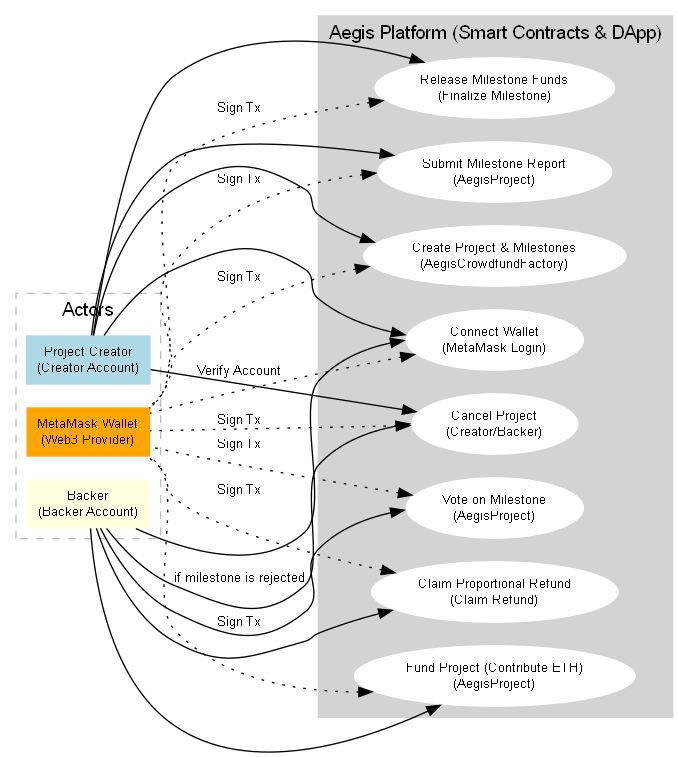
\includegraphics[width=0.85\textwidth]{use-case-en.png}
\caption{Use Case Diagram Aegis}
\label{fig:usecase}
\end{figure}
\clearpage

\clearpage
\subsection{Activity Diagram}
Activity diagram menggambarkan alur kontribusi hingga release dana, termasuk percabangan ketika milestone ditolak atau deadline terlewati.
\begin{figure}[h]
\centering
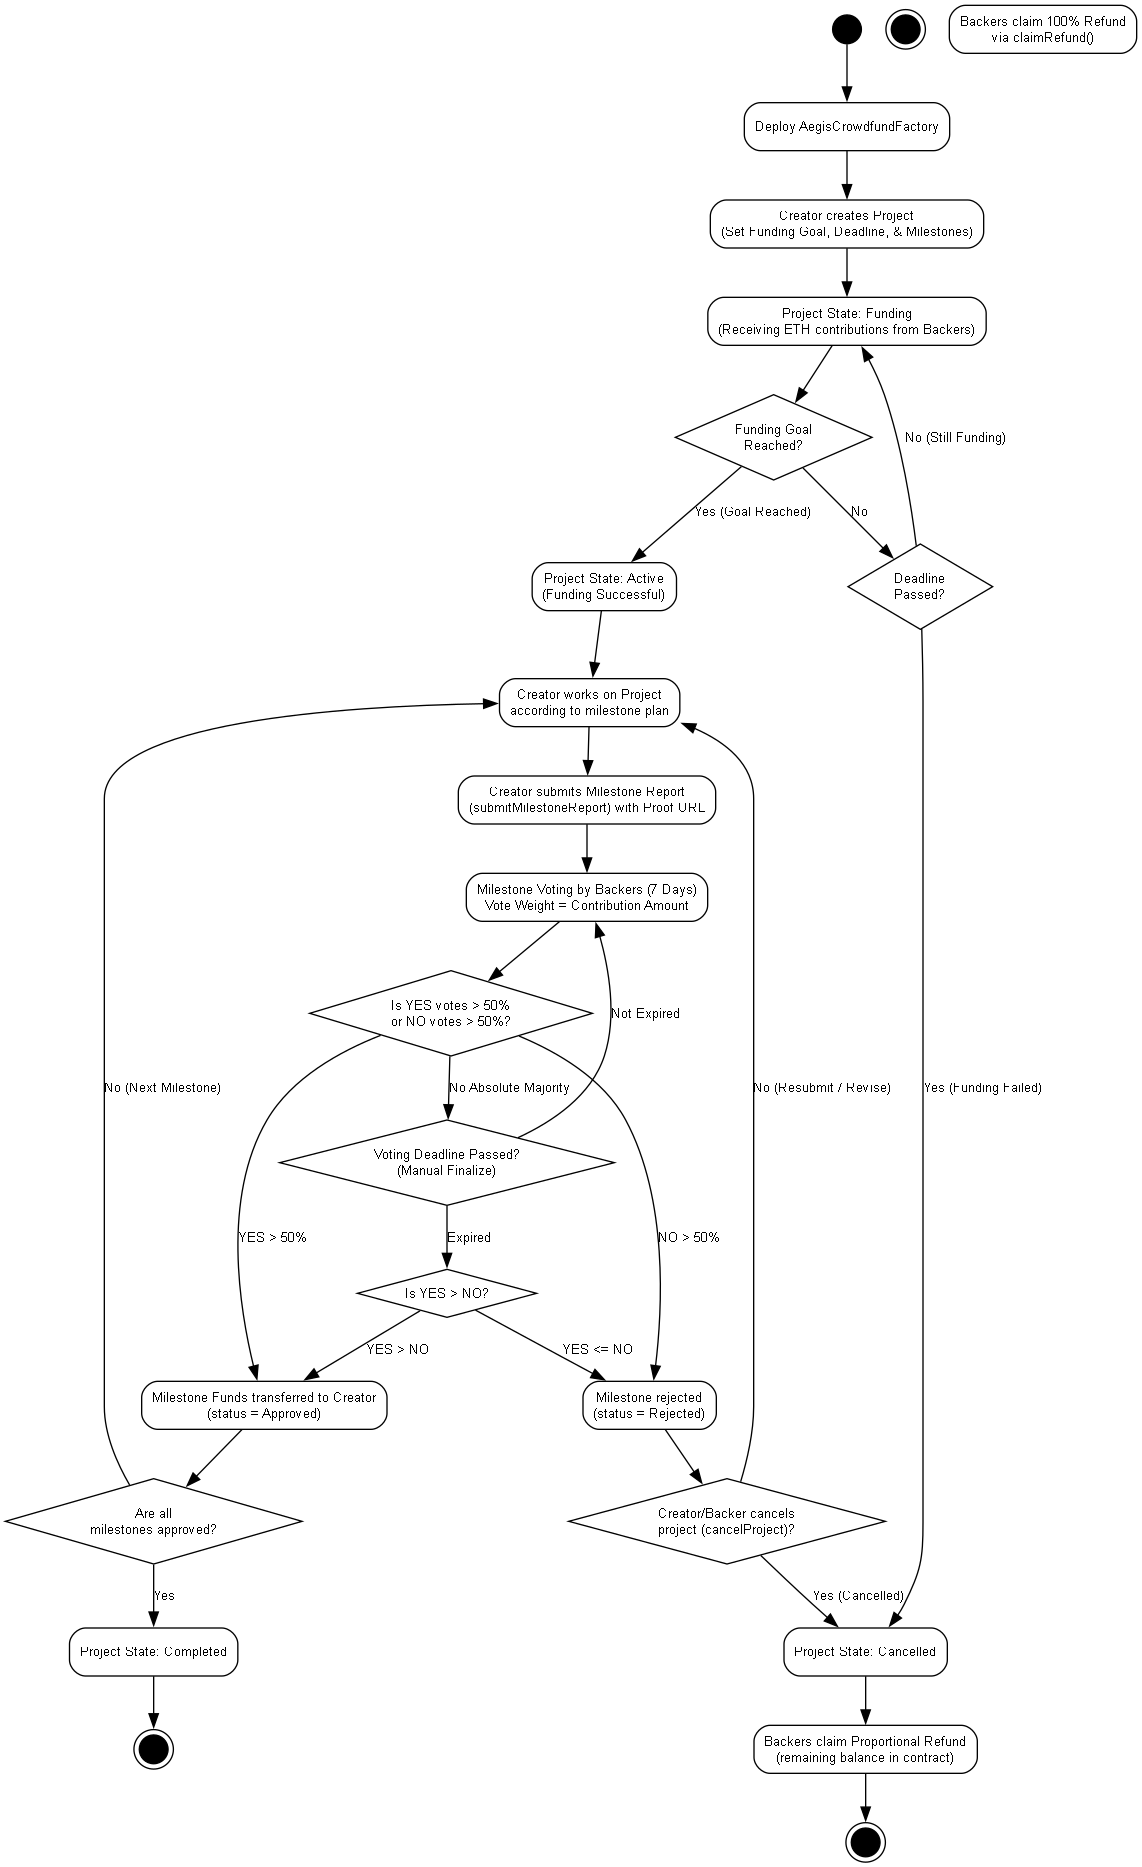
\includegraphics[width=0.7\textwidth]{activity-en.png}
\caption{Activity Diagram Alur Crowdfunding}
\label{fig:activity}
\end{figure}
\clearpage

\clearpage
\subsection{Sequence Diagram}
Sequence diagram menekankan urutan pesan antara UI, wallet, dan smart contract ketika transaksi dikirim dan dikonfirmasi.
\begin{figure}[h]
\centering
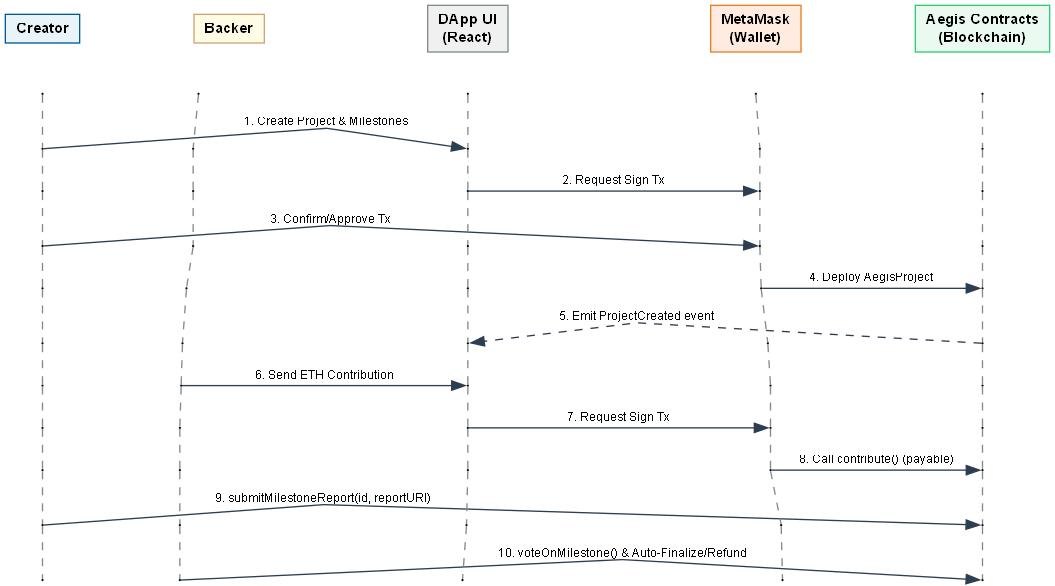
\includegraphics[width=1\textwidth]{sequence-en.png}
\caption{Sequence Diagram Interaksi UI--Wallet--Smart Contract}
\label{fig:sequence}
\end{figure}
\clearpage

\clearpage
\subsection{Class Diagram / ERD}
Diagram kelas/ERD digunakan untuk memetakan struktur data kontrak (Project, Milestone, Backer) dan relasi antar entitas.
\begin{figure}[h]
\centering
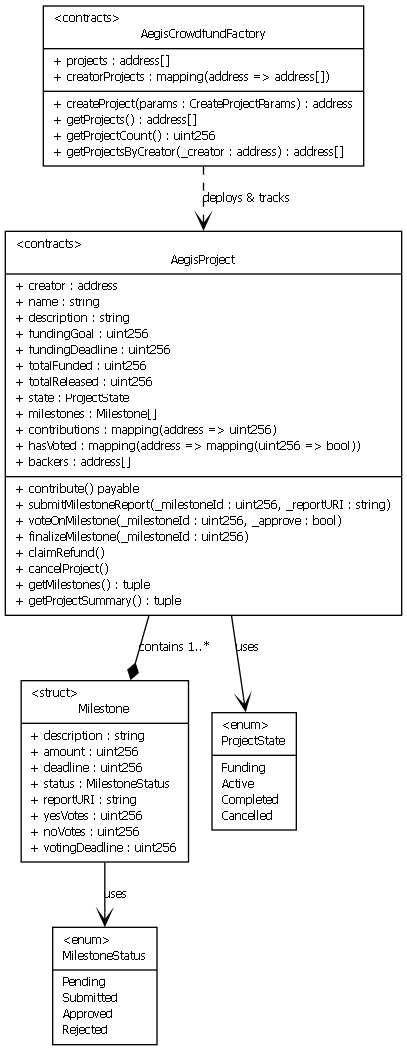
\includegraphics[width=0.4\textwidth]{erd-en.png}
\caption{Class Diagram / ERD Struktur Data Aegis}
\label{fig:erd}
\end{figure}
\clearpage

\subsection{Desain Database}
Tidak ada database off-chain pada tahap ini. Seluruh status proyek, milestone, dan kontribusi disimpan on-chain dalam smart contract.

\clearpage
\subsection{Desain Antarmuka}
Mockup antarmuka mencakup landing page, halaman eksplorasi proyek, detail proyek, dan manajemen proyek kreator. Komponen kunci meliputi kartu proyek, progress bar pendanaan, dan panel milestone.
\begin{figure}[h]
\centering
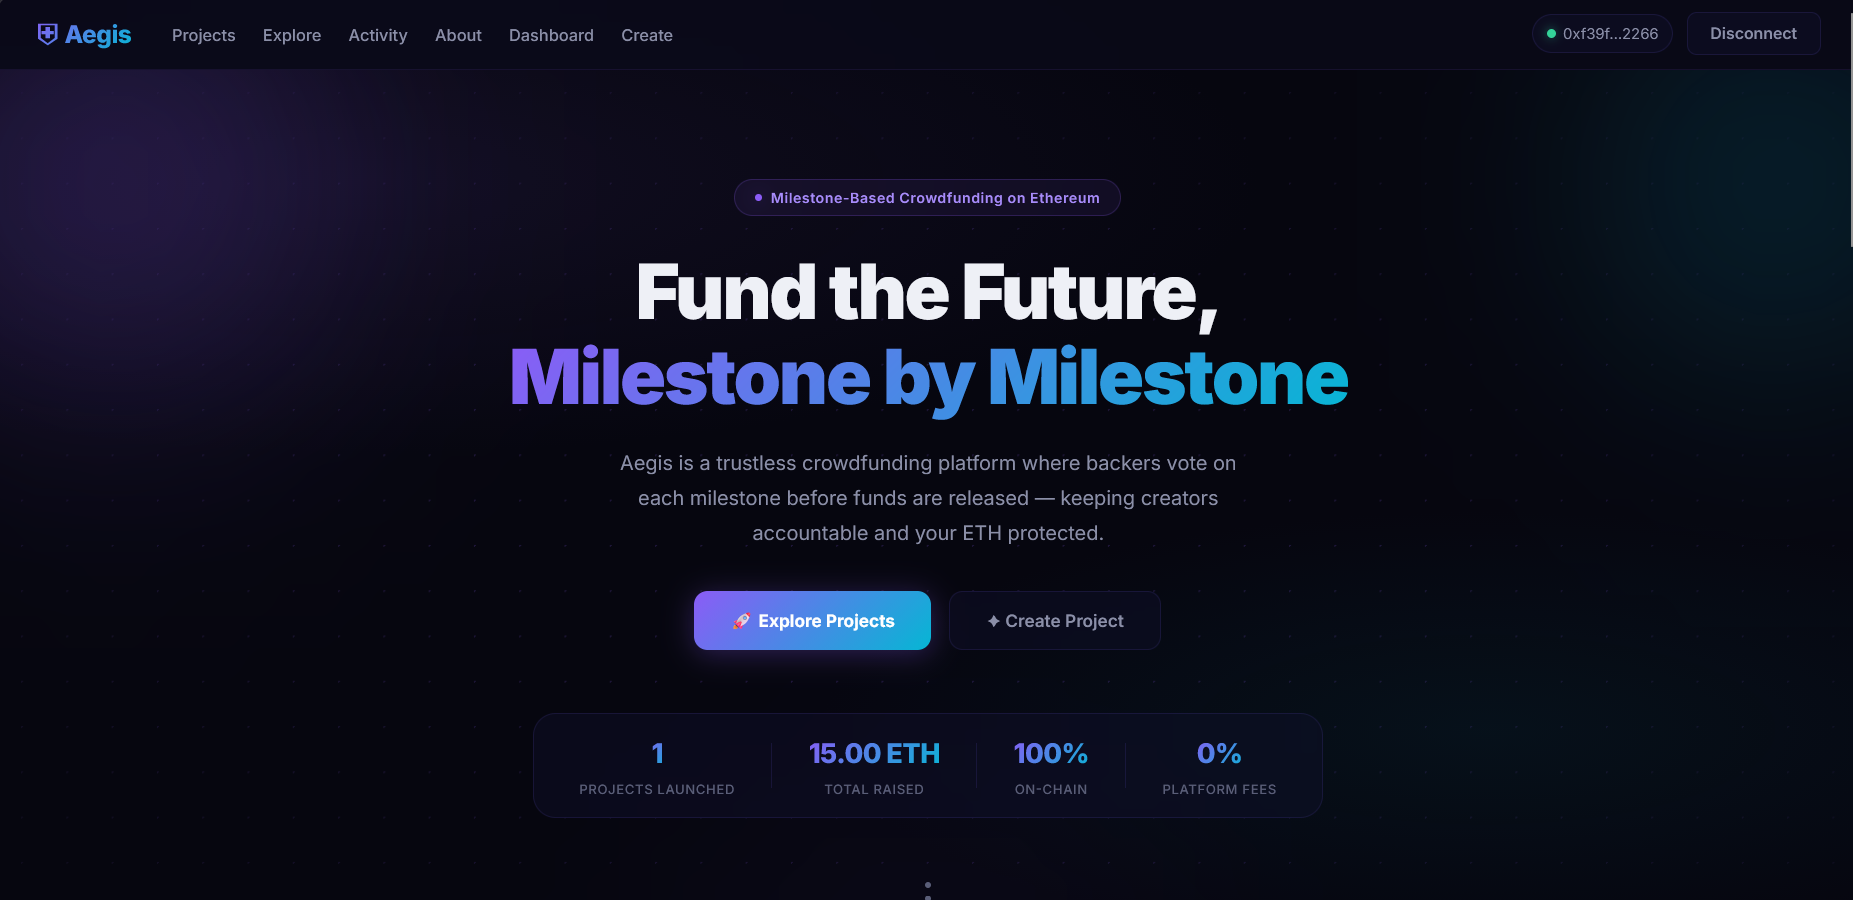
\includegraphics[width=0.6\textwidth]{photos/mockup-antarmuka.png}
\caption{Mockup Antarmuka Utama}
\label{fig:ui-mockup}
\end{figure}
\clearpage

\section{BAB 5. MANAJEMEN PROYEK}
\subsection{Struktur Tim}
Tim terdiri dari 3 anggota dengan pembagian objektif yang setara berdasarkan modul.

\subsection{Pembagian Tugas}
\begin{longtable}{p{0.24\textwidth} p{0.7\textwidth}}
\toprule
\textbf{Anggota} & \textbf{Objektif Utama (Setara)} \\
\midrule
Rifqi Ramadhan & Smart contract core (Factory + Project), alur milestone, dan integrasi deploy. \\
George Wiliam Thomas Gonata & Logika voting berbasis kontribusi, validasi milestone, dan pengujian voting/refund. \\
Samuel Tanaka Sibarani & Frontend React, Web3 context, dan integrasi flow UI (create, vote, finalize). \\
\bottomrule
\end{longtable}

\subsection{Jadwal Proyek}
\begin{longtable}{p{0.22\textwidth} p{0.73\textwidth}}
	\toprule
	\textbf{Periode} & \textbf{Kegiatan} \\
\midrule
Akhir Jan 2026 & R\&D awal: studi literatur crowdfunding berbasis blockchain dan milestone release. \\
Feb 2026 (Minggu 1--2) & Perancangan arsitektur: pemisahan Factory--Project, perumusan state project, dan definisi milestone. \\
Feb 2026 (Minggu 3--4) & Prototipe flow crowdfunding: kontribusi ETH, milestone report, dan refund logic. \\
Maret 2026 (Minggu 1--2) & Desain voting: bobot suara berbasis kontribusi dan auto-finalize saat mayoritas tercapai. \\
Maret 2026 (Minggu 3--4) & Konsolidasi desain dan revisi modul smart contract sebelum fase implementasi. \\
Awal Apr 2026 & Implementasi kontrak inti: \texttt{AegisCrowdfundFactory} dan \texttt{AegisProject}. \\
Pertengahan Apr 2026 & Integrasi frontend awal: Home, Create Project, Project Detail. \\
Akhir Apr 2026 & Penambahan layout, routing, dan halaman eksplorasi (Landing, Explore, About, Guide). \\
Awal Mei 2026 & Dashboard pengguna, halaman aktivitas, profil, dan halaman manajemen proyek creator. \\
Pertengahan Mei 2026 & Pengujian smart contract: workflow crowdfunding, voting, refund, dan completion. \\
\bottomrule
\end{longtable}

\subsection{Manajemen Risiko Proyek}
Pada tahap prototipe, risiko utama berada pada dua lapisan: logika kontrak dan perilaku pengguna. Dari sisi kontrak, risiko terbesar adalah pelepasan dana yang tidak sesuai progres. Mitigasinya adalah alur milestone yang mengharuskan laporan dibuat terlebih dahulu, diikuti voting yang mengunci keputusan komunitas sebelum dana dilepas. Auto-finalize hanya terjadi ketika mayoritas tercapai, sehingga menghindari pencairan tanpa konsensus.

Risiko kedua berkaitan dengan konsentrasi suara karena bobot voting berbasis kontribusi. Dalam skenario backer sedikit, keputusan bisa didominasi pihak tertentu. Mitigasi jangka pendek adalah transparansi: kontribusi dan hasil voting dapat dilihat oleh semua pihak, serta milestone dapat ditolak jika bukti tidak memadai. Mitigasi jangka panjang yang direncanakan adalah migrasi ke governance token dengan delegasi suara untuk memperluas partisipasi.

Risiko operasional muncul pada integrasi wallet dan UX transaksi. Pengguna dapat mengalami kegagalan transaksi akibat gas atau salah jaringan. UI menampilkan status transaksi dan menyediakan umpan balik setelah konfirmasi, sementara konfigurasi lokal menggunakan Hardhat node untuk mengurangi risiko gagal transaksi pada tahap pengujian.

Terakhir, risiko ekosistem terkait volatilitas ETH. Karena kontribusi masih menggunakan ETH, nilai dana dapat berfluktuasi. Mitigasi yang direncanakan adalah penggunaan stablecoin escrow serta integrasi DeFi yield agar dana idle tetap produktif tanpa mengorbankan stabilitas nilai.

\subsection{Estimasi Biaya dan Infrastruktur}
Estimasi biaya difokuskan pada gas fee transaksi dan kebutuhan infrastruktur pengujian. Pada tahap prototipe, biaya diminimalkan dengan penggunaan jaringan lokal Hardhat, sehingga eksekusi transaksi tidak memerlukan biaya riil. Untuk tahap lanjut, kebutuhan biaya mencakup deployment testnet/mainnet, hosting frontend, serta biaya operasional node atau RPC provider.

\section{BAB 6. IMPLEMENTASI SISTEM}
Bagian ini menjelaskan implementasi aktual yang dikerjakan oleh tim dalam satu alur pengembangan. Selain kontrak inti, perubahan terbesar terjadi pada layer frontend: routing multi-halaman, dashboard pengguna, dan halaman manajemen proyek untuk kreator.

\subsection{Lingkungan Pengembangan}
Pengembangan dilakukan pada OS desktop dengan tool utama: Hardhat untuk smart contract, React + Vite untuk frontend, dan MetaMask sebagai wallet. Node lokal Hardhat digunakan untuk pengujian deterministik.

\subsection{Implementasi Smart Contract}
Implementasi kontrak berfokus pada ketertelusuran status proyek dan alur dana. Kontrak project menyimpan milestone, membuka voting saat report masuk, dan menutup voting ketika mayoritas tercapai atau deadline lewat. Auto-finalize membantu menghindari penundaan pencairan pada skenario demo dengan backer terbatas. Pada saat yang sama, mekanisme refund menjaga hak backer ketika proyek dibatalkan atau deadline pendanaan terlewati.
\begin{itemize}[leftmargin=1.2em]
  \item \texttt{AegisCrowdfundFactory.sol}: deploy proyek dan registry.
  \item \texttt{AegisProject.sol}: contribute ETH, submit report, vote, finalize, refund, cancel.
  \item Voting berbasis kontribusi diterapkan di \texttt{AegisProject.sol}.
\end{itemize}

\subsection{Ringkasan Fungsi Kontrak}
Rangkuman berikut membantu menghubungkan fungsi utama dengan kebutuhan fungsional yang telah didefinisikan. Semua fungsi bersifat on-chain dan dapat dipanggil langsung dari UI melalui MetaMask.
\begin{itemize}[leftmargin=1.2em]
  \item \textbf{AegisCrowdfundFactory}: \texttt{createProject()}, \texttt{getProjects()}, \texttt{getProjectCount()}, \texttt{getProjectsByCreator()}.
  \item \textbf{AegisProject}: \texttt{contribute()}, \texttt{submitMilestoneReport()}, \texttt{voteOnMilestone()}, \texttt{finalizeMilestone()}, \texttt{claimRefund()}, \texttt{cancelProject()}, \texttt{getMilestones()}, \texttt{getMilestoneCount()}, \texttt{getBackers()}, \texttt{getContractBalance()}, \texttt{getProjectSummary()}.
  \item \textbf{AegisProject}: \texttt{voteOnMilestone()} menggunakan bobot kontribusi \texttt{contributions}.
\end{itemize}

\subsection{Implementasi Frontend}
Layer frontend berperan sebagai antarmuka pengguna untuk membaca state kontrak dan mengeksekusi transaksi. Perubahan pada branch ini menekankan pengalaman pengguna: landing page, pencarian proyek, dashboard personal, hingga halaman manajemen khusus kreator. Prinsip desainnya adalah mengurangi friksi transaksi dengan tampilan status yang jelas, feedback ketika transaksi dikirim, serta navigasi yang konsisten antara halaman eksplorasi dan halaman detail.
\begin{itemize}[leftmargin=1.2em]
  \item \texttt{Landing.jsx}: landing page dengan statistik proyek.
  \item \texttt{Home.jsx}: eksplorasi proyek dengan pencarian dan filter.
  \item \texttt{CreateProject.jsx}: form pembuatan proyek + milestones.
  \item \texttt{ProjectDetail.jsx}: contribute, submit report, vote, finalize.
  \item \texttt{ProjectManage.jsx}: dashboard khusus creator untuk kelola milestone.
  \item \texttt{Dashboard.jsx}: ringkasan proyek dibuat dan didukung pengguna.
  \item \texttt{Web3Context.jsx}: koneksi MetaMask, signer/provider, kontrak factory/project.
\end{itemize}

\subsection{Integrasi Sistem}
Pada sisi backer, perjalanan dimulai dari halaman \texttt{Landing} untuk memahami konsep dan statistik proyek yang telah berjalan. Setelah terhubung melalui MetaMask, backer dapat mencari proyek di \texttt{Home}, membaca detail pada \texttt{ProjectDetail}, dan mengirim kontribusi ETH. Ketika kreator mengajukan laporan milestone, backer meninjau bukti (URL, gambar, atau video) yang ditampilkan di UI lalu memberikan suara. Bobot suara ditentukan oleh kontribusi, sehingga keputusan pendanaan mencerminkan risiko finansial yang diambil.

Pada sisi kreator, alur dimulai dari \texttt{CreateProject} untuk mendefinisikan target pendanaan dan milestone. Setelah pendanaan tercapai, kreator mengunggah laporan milestone secara bertahap. Halaman \texttt{ProjectManage} menyediakan ringkasan status, jumlah milestone yang pending/approved, serta kontrol untuk membatalkan proyek jika diperlukan. Dengan alur ini, kreator dan backer memiliki konteks yang sama terhadap status proyek dan keputusan pencairan dana.

\subsection{Fitur UI yang Menonjol}
Fitur UI dirancang untuk memberi konteks dan kepercayaan bagi backer, sekaligus memberi alat eksekusi yang jelas bagi kreator. Fokusnya adalah membuat informasi kritikal (status proyek, target pendanaan, dan hasil voting) terlihat tanpa harus membaca data mentah on-chain.
\begin{itemize}[leftmargin=1.2em]
  \item Proof builder: laporan milestone dapat berupa URL, image, video, atau teks (diserialisasi ke JSON).
  \item Proof viewer: render proof dan lightbox untuk bukti berbasis gambar/video.
  \item Routing multi-halaman dengan layout terpisah (Landing/Main) dan ErrorBoundary.
  \item Dashboard aktivitas: statistik proyek, kontribusi, dan status milestone.
\end{itemize}

\subsection{Pemetaan Fitur ke File Implementasi}
\begin{longtable}{p{0.28\textwidth} p{0.66\textwidth}}
	\toprule
	\textbf{Fitur} & \textbf{File Utama} \\
	\midrule
Pembuatan proyek & \texttt{frontend/src/pages/CreateProject.jsx}, \texttt{contracts/AegisCrowdfundFactory.sol} \\
Funding dan status proyek & \texttt{frontend/src/pages/ProjectDetail.jsx}, \texttt{contracts/AegisProject.sol} \\
Voting milestone & \texttt{frontend/src/pages/ProjectDetail.jsx}, \texttt{contracts/AegisProject.sol} \\
Manajemen proyek kreator & \texttt{frontend/src/pages/ProjectManage.jsx} \\
Dashboard pengguna & \texttt{frontend/src/pages/Dashboard.jsx} \\
Landing + eksplorasi proyek & \texttt{frontend/src/pages/Landing.jsx}, \texttt{frontend/src/pages/Home.jsx} \\
Routing & \texttt{frontend/src/App.jsx}, \texttt{frontend/src/layouts/MainLayout.jsx}, \texttt{frontend/src/layouts/LandingLayout.jsx} \\
Web3 connectivity & \texttt{frontend/src/context/Web3Context.jsx} \\
Pengujian kontrak & \texttt{test/AegisProject.test.js} \\
Deployment lokal & \texttt{ignition/modules/AegisFactory.js}, \texttt{hardhat.config.js} \\
\bottomrule
\end{longtable}

\subsection{Implementasi Backend/API}
Sistem tidak menggunakan backend terpisah. Semua state utama berada di smart contract, sementara frontend berperan sebagai klien yang melakukan pembacaan dan transaksi on-chain.

\subsection{Implementasi Wallet dan Web3}
Integrasi wallet dilakukan melalui MetaMask. Modul \texttt{Web3Context} mengelola koneksi akun, signer, dan instans kontrak agar UI dapat memanggil fungsi on-chain secara konsisten.

\subsection{Deployment Blockchain}
Deployment dilakukan pada jaringan lokal Hardhat menggunakan Ignition. Pendekatan ini memudahkan pengujian tanpa biaya gas riil dan memungkinkan pengulangan skenario secara konsisten.

\section{BAB 7. PENGUJIAN DAN EVALUASI}
\subsection{Skenario Pengujian}
Skenario pengujian mencakup pembuatan proyek, kontribusi hingga target tercapai, submit milestone, voting, finalize milestone, serta refund jika proyek dibatalkan atau deadline terlewati.

\subsection{Functional Testing}
Pengujian fungsional memastikan setiap fitur berjalan sesuai kebutuhan: create project, contribute, vote, finalize, dan refund. Hasil pengujian dicatat melalui test suite Hardhat.

\subsection{Smart Contract Testing}
Pengujian kontrak dilakukan dengan Hardhat melalui \texttt{AegisProject.test.js} yang memverifikasi alur funding, voting, dan completion.

\subsection{Performance Testing}
Uji performa difokuskan pada biaya gas dan waktu eksekusi transaksi pada jaringan lokal. Hasil ini digunakan sebagai baseline sebelum uji testnet.

\subsection{Security Evaluation}
Evaluasi keamanan memeriksa potensi celah pada proses voting dan release dana. Mekanisme auto-finalize hanya terjadi pada mayoritas, sementara refund memastikan backer terlindungi pada kondisi gagal.

\subsection{User Acceptance Testing (UAT)}
UAT dilakukan melalui simulasi end-to-end oleh tim: pembuatan proyek, pendanaan, submit report, voting, dan pencairan dana.

\subsection{Evaluasi Hasil}
Secara umum, hasil pengujian menunjukkan bahwa alur inti berfungsi dengan konsisten pada jaringan lokal, dengan UI yang mampu menampilkan status proyek secara jelas.

\section{BAB 8. HASIL DAN TAMPILAN LUARAN SISTEM}
Bagian ini menyajikan ringkasan tampilan utama yang direkomendasikan untuk ditambahkan sebagai lampiran screenshot.
\subsection{Tampilan Dashboard}
Tampilan dashboard menampilkan proyek yang dibuat/didanai, status milestone, dan ringkasan kontribusi.
\begin{figure}[h]
\centering
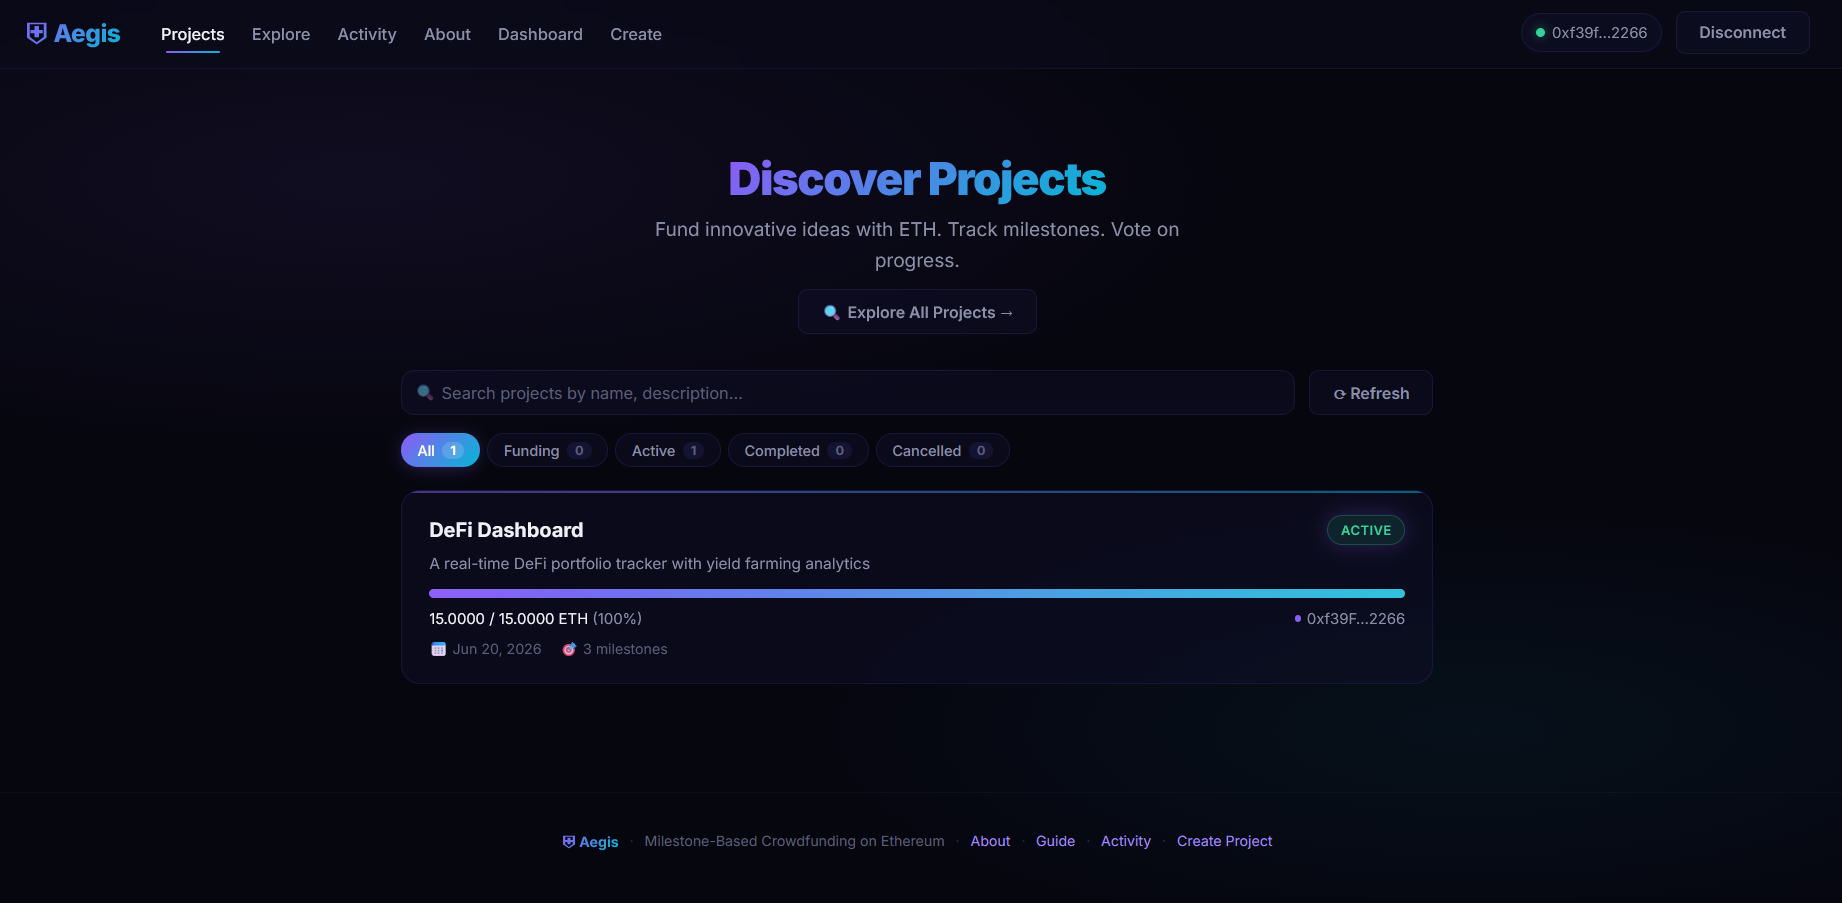
\includegraphics[width=0.9\textwidth]{photos/screenshot-dashboard.png}
\caption{Tampilan Dashboard Pengguna}
\label{fig:dashboard}
\end{figure}

\subsection{Tampilan Transaksi Blockchain}
Transaksi dicatat on-chain dan dapat divisualisasikan melalui status di UI atau explorer lokal.
\begin{figure}[h]
\centering
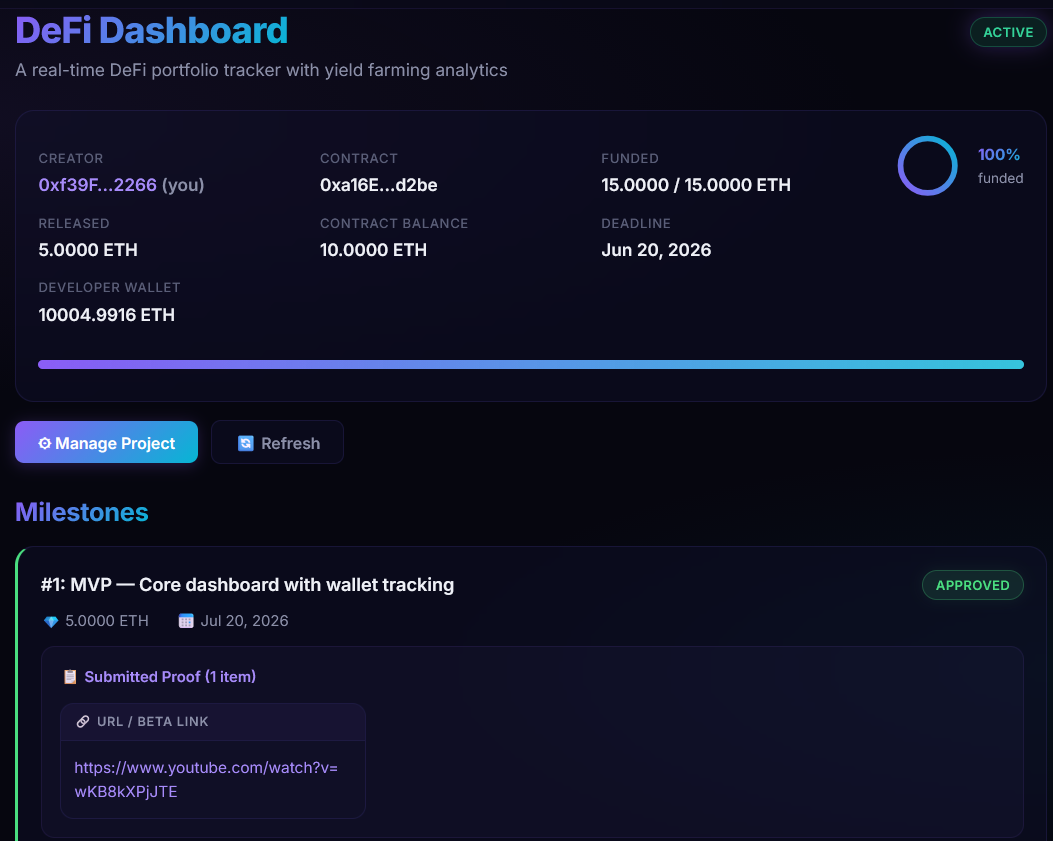
\includegraphics[width=0.6\textwidth]{photos/screenshot-transaksi.png}
\caption{Tampilan Transaksi On-Chain}
\label{fig:tx}
\end{figure}

\subsection{Analisis Kelebihan Sistem}
Kelebihan utama adalah transparansi status proyek dan mekanisme kontrol komunitas terhadap pencairan dana.

\subsection{Analisis Kekurangan Sistem}
Kekurangan utama adalah ketergantungan pada ETH dan belum adanya governance token.

\section{BAB 9. KESIMPULAN DAN SARAN}
\subsection{Kesimpulan}
Secara keseluruhan, Aegis sudah mencapai fase fungsional end-to-end untuk crowdfunding milestone berbasis kontribusi. Sistem membuktikan bahwa milestone report dan voting dapat dijalankan sepenuhnya on-chain, sementara frontend menyediakan konteks yang cukup untuk keputusan backer dan tindakan kreator.

\subsection{Kontribusi Project}
Kontribusi proyek adalah penyediaan prototipe end-to-end yang dapat menjadi basis pengembangan governance lebih lanjut serta studi penggunaan smart contract untuk akuntabilitas crowdfunding.

\subsection{Saran Pengembangan}
Saran utama mencakup stablecoin escrow, DeFi yield, dan governance token dengan delegated voting.

\subsection{Fitur Belum Diimplementasikan}
\begin{itemize}[leftmargin=1.2em]
  \item Escrow stablecoin (USDC/USDT) menggantikan ETH.
  \item Integrasi DeFi yield (Aave/Compound) untuk idle funds.
  \item Modul governance token terpisah dan snapshot voting.
  \item Treasury DAO dan proposal governance penuh.
\end{itemize}

\subsection{Keterbatasan Saat Ini}
Pada tahap ini, model governance masih bergantung pada kontribusi ETH dan belum mendukung representasi kepemilikan berbasis token atau delegated voting. Selain itu, tidak ada modul risk guard (misalnya AI sentiment) maupun integrasi DeFi untuk optimalisasi dana. Keterbatasan ini disengaja agar fokus implementasi tetap pada alur inti dan pengalaman pengguna.

\section*{Daftar Pustaka}
\begin{thebibliography}{25}

\bibitem{juicebox}
Juicebox DAO, ``Juicebox Protocol Documentation,'' 2026. [Online]. Available: \url{https://docs.juicebox.money/} Accessed: Jun. 2026.

\bibitem{hybridai}
B. S. Lakshmi and K. S. Rekha, ``A Hybrid Blockchain--AI Architecture for Secure and Transparent Decentralized Crowdfunding,'' \textit{Journal of Artificial Intelligence and Technology}, vol. 5, pp. 557--562, Nov. 2025, doi: 10.37965/jait.2025.0834.

\bibitem{ethereum}
V. Buterin, ``Ethereum Whitepaper,'' 2014. [Online]. Available: \url{https://ethereum.org/en/whitepaper/}

\bibitem{hardhat}
Nomic Foundation, ``Hardhat Ethereum Development Environment,'' 2026. [Online]. Available: \url{https://hardhat.org/docs} Accessed: Jun. 2026.

\bibitem{metamask}
MetaMask, ``MetaMask Documentation,'' 2026. [Online]. Available: \url{https://docs.metamask.io/} Accessed: Jun. 2026.

\bibitem{rathore2023decentralized}
A. Rathore and S. W. A. Rizvi, ``Decentralized Crowdfunding Platform Using Blockchain,'' \textit{Journal of Informatics Electrical and Electronics Engineering}, 2023, doi: 10.54060/jieee.2023.79.

\bibitem{jayapal2023capitalizing}
C. Jayapal, A. R. Xavier, and P. Arunachalam, ``Capitalizing on Blockchain Technology for Efficient Crowdfunding: An Exploration of Ethereum's Smart Contracts,'' \textit{International Journal of Safety and Security Engineering}, vol. 13, no. 4, pp. 723--729, 2023, doi: 10.18280/ijsse.130415.

\bibitem{aprialim2021penerapan}
F. Aprialim, Adnan, and A. W. Paundu, ``Penerapan Blockchain dengan Integrasi Smart Contract pada Sistem Crowdfunding,'' \textit{Jurnal RESTI}, vol. 5, no. 1, pp. 148--154, 2021, doi: 10.29207/resti.v5i1.2613.

\bibitem{ahmad2021applying}
N. A. N. Ahmad and S. A. H. Rahman, ``Applying Ethereum Smart Contracts to Blockchain-Based Crowdfunding System to Increase Trust and Information Symmetry,'' in \textit{ICCTA 2021}, 2021, doi: 10.1145/3477911.3477920.

\bibitem{zichichi2019likestarter}
M. Zichichi, M. Contu, S. Ferretti, and G. D'Angelo, ``LikeStarter: A Smart-contract based Social DAO for Crowdfunding,'' in \textit{IEEE INFOCOM Workshops}, 2019, doi: 10.1109/INFCOMW.2019.8845133.

\bibitem{shelke2022blockchain}
P. Shelke, S. Zanjal, R. Patil, and D. Desai, ``Blockchain Technology Based Crowdfunding Using Smart Contracts,'' in \textit{ICAISS}, 2022, pp. 939--943, year={2022}, doi: 10.1109/ICAISS55157.2022.10010749.

\bibitem{bitfund2020}
``BitFund: A Blockchain-Based Crowd Funding Platform for Future Smart and Connected Nation,'' \textit{Sustainable Cities and Society}, vol. 60, p. 102145, 2020, doi: 10.1016/j.scs.2020.102145.

\bibitem{alruwaili2020milestone}
A. Alruwaili and D. Kruger, ``Crowdfunding with Periodic Milestone Payments Using a Smart Contract to Implement Fair E-Voting,'' in \textit{Business Information Systems Workshops}, 2020, pp. 61--72, doi: 10.1007/978-3-030-61146-0\_5.

\bibitem{villanueva2025metamorphic}
I. J. Villanueva, M. Srinivasan, and F. ur Rehman, ``Metamorphic Testing for Smart Contract Validation: A Case Study of Ethereum-Based Crowdfunding Contracts,'' \textit{SANER}, 2025, pp. 97--105, doi: 10.1109/SANER-C66551.2025.00021.

\bibitem{chen2023dcc}
B. Chen, Y. Luo, J. Li, \textit{et al.}, ``Blockchain-Based Decentralized Co-governance: Innovations and Solutions for Sustainable Crowdfunding,'' \textit{arXiv preprint arXiv:2306.00869}, 2023.

\bibitem{nakamoto2008bitcoin}
S. Nakamoto, ``Bitcoin: A Peer-to-Peer Electronic Cash System,'' 2008.

\bibitem{openzeppelin}
OpenZeppelin, ``OpenZeppelin Smart Contract Library,'' 2026. [Online]. Available: \url{https://openzeppelin.com/} Accessed: Jun. 2026.

\bibitem{ethersjs}
R. Moore, ``Ethers.js Documentation,'' 2026. [Online]. Available: \url{https://docs.ethers.org/} Accessed: Jun. 2026.

\bibitem{react}
Meta, ``React Documentation,'' 2026. [Online]. Available: \url{https://react.dev/} Accessed: Jun. 2026.

\bibitem{solidity}
Solidity Team, ``Solidity Documentation,'' 2026. [Online]. Available: \url{https://docs.soliditylang.org/} Accessed: Jun. 2026.

\bibitem{wood2015ethereum}
G. Wood, ``Ethereum: A Secure Decentralised Generalised Transaction Ledger,'' \textit{Ethereum Project Yellow Paper}, vol. 151, pp. 1--32, 2015.

\bibitem{szabo1997formalizing}
N. Szabo, ``Formalizing and Securing Relationships on Public Networks,'' \textit{First Monday}, vol. 2, no. 9, 1997.

\bibitem{dhillon2017blockchain}
V. Dhillon, D. Metcalf, and M. Hooper, ``Blockchain Enabled Crowdfunding,'' in \textit{Blockchain Enabled Applications}, Apress, pp. 3--21, 2017.

\bibitem{vogel2023smart}
T. Vogel, ``Smart Contract Vulnerabilities: A Survey on Security Attacks and Countermeasures,'' \textit{arXiv preprint arXiv:2303.01122}, 2023.

\bibitem{pasolini2022daos}
E. Pasolini, ``Decentralized Autonomous Organizations (DAOs): A Governance Framework for Crowdfunding,'' \textit{Journal of Corporate Finance and Governance}, 2022.

\end{thebibliography}

\end{document}
